\comment{Suggestion: past tense}\\

\subsection{Gradient Descent analysis}
    \begin{figure*}
        \begin{subfigure}{.5\textwidth}
            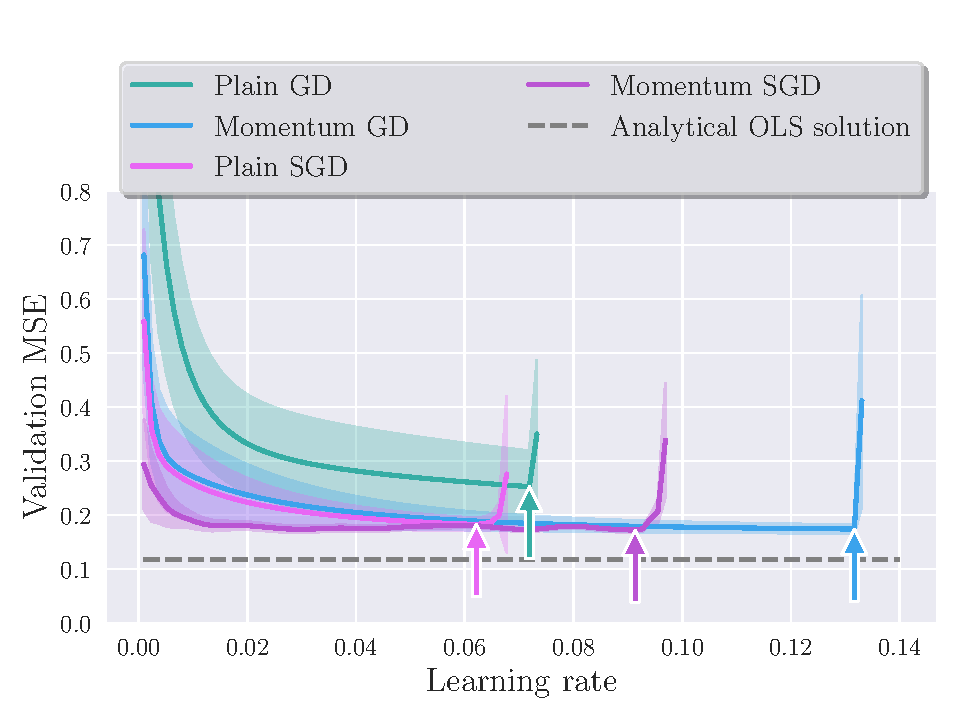
\includegraphics[width=\linewidth]{learning_rates_PGD_MGD_PSGD_MSGD.pdf}
            \caption{Best MSEs, learning rates: (0.2990, 0.0655), (0.1823, 0.122), (0.2006, 0.0165), (0.1975, 0.0358)}
            \label[fig]{res:fig:lrate1}
        \end{subfigure}
        \hfill
        \begin{subfigure}{.5\textwidth}
            \centering
            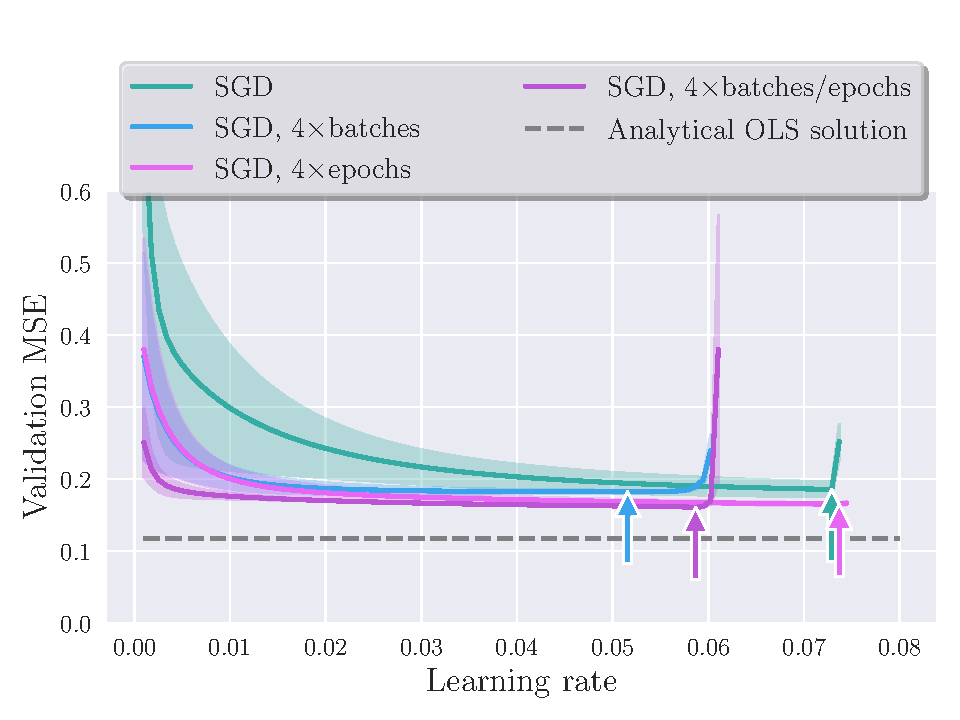
\includegraphics[width=\linewidth]{learning_rates_SGD_batches_epochs.pdf}
            \caption{Best MSEs, learning rates: (0.1865, 0.0405), (0.1803, 0.129), (0.1781, 0.293)}
            \label[fig]{res:fig:lrate2}
        \end{subfigure}
        \hfill
        \begin{subfigure}{.5\textwidth}
            \centering
            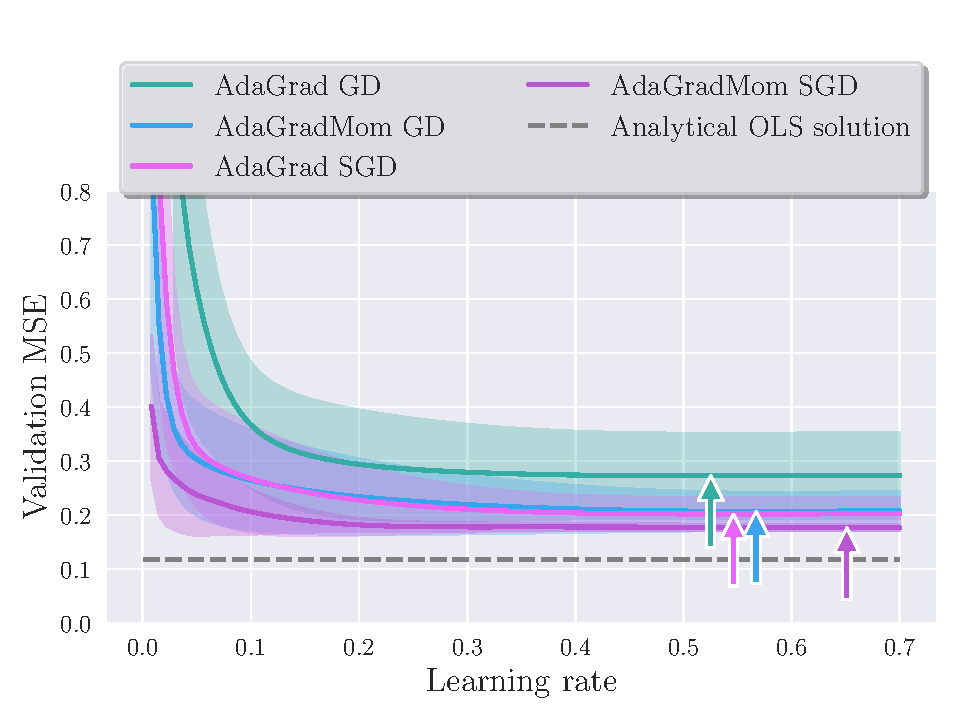
\includegraphics[width=\linewidth]{learning_rates_adagrad}
            \caption{Best MSEs, learning rates: (0.3185, 0.498), (0.2312, 0.576), (0.1970, 0.139), (0.1964, 0.43)}
            \label[fig]{res:fig:lrate3}
        \end{subfigure}
        \caption{Plots of the validation MSE of the parameters found from optimising the OLS cost function on Franke function data with $n=600$ data points. For the momentum methods we used $\gamma=0.8$. The stochastic methods used 32 batches and 100 epochs, while the standard GD did 100 iterations unless specified otherwise.}
        \label[fig]{res:fig:lrates}
    \end{figure*}